\documentclass[11pt,letterpaper]{article}
\usepackage{naaclhlt2010}
\usepackage{times}
\usepackage{graphicx}
\usepackage{latexsym}
\setlength\titlebox{6.5cm}

\title{EN.600.461 Computer Vision\\Final Project\\Recognizing and Translating Text from Images}

\author{Joon Hyuck (James) Choi\\
  \textit{Senior Undergraduate}\\
  The Johns Hopkins University\\
  3400 N Charles Street\\
  Baltimore, MD 21218, USA\\
  {\tt jchoi100@jhu.edu}}

\date{Dec X, 2016}

\begin{document}
\maketitle
\begin{abstract}
  This work explores optical character recognition (OCR) in photos of typed and handwritten documents. It first explores basic preprocessing of photos of documents using {\tt OpenCV} \footnote{http://opencv.org/} functionalities for blurring, thresholding, and denoising. It next discusses the use of {\tt tesseract-ocr} \footnote{https://github.com/tesseract-ocr} to perform OCR. We then discuss the incorporation of the Google Cloud Translation API \footnote{https://cloud.google.com/translate/} to translate the OCR results into different languages. It finally discusses template matching using the Johns Hopkins University (JHU) logo and signatures of three U.S. presidents on sample document images. 
\end{abstract}

\section{Introduction}

This work achieved the following main goals stated in the original proposal: 1) Given a photo of a document, convert it into a clean scanned version; 2) Take the scanned version and perform OCR. Optionally, this work took the OCR output and translated the text into different languages using the Google Cloud Translation API. This work also experimented with template matching using the JHU logo in order to determine whether the input document is an official JHU document or not. Lastly, this work performed CNN training on the MNIST handwritten digit dataset as an experiment.

\section{Dataset}

\subsection{Typed Documents}

We took photos of the final project guidelines for this course, the author's project proposal, JHU's Lav Note, and four aesop's fables, which the author typed and printed in different font types and sizes. A sample input image is shown in Figure 2.

\subsection{Handwritten Documents}

We collected photos of letters written by three U.S. presidents, Barack Obama, George W. Bush, and Bill Clinton. We also hand-wrote portions of the aesop's fables mentioned above with different handwriting, photographed under different settings. Figure 3 shows one of our reasonably neat images {\tt hand\textunderscore cat.png}, and Figure 4 shows a sample letter written by Preisdent Obama.

\subsection{Templates}

For the template mathcing experiments, we collected images of the JHU logo in several sizes and signatures of the three U.S. presidents listed above.

\section{Methods}

In this section, we discuss the methods we took and external libraries used for each stage of our work.

\subsection{Image Preprocessing}

We implemented our program in Python using {\tt OpenCV}. In order to feed the OCR algorithm clean input to achieve best performance, we used {\tt cv2.medianBlur} to smoothen the input image with an aperture size of 5. Then, we performed binary thresholding on the smoothened image using {\tt cv2.adaptiveThreshold} with \textit{adaptiveMethod=} \textit{ ADAPTIVE\textunderscore THRESH\textunderscore GAUSSIAN\textunderscore C}, \textit{threshold = binary}, \textit{blockSize=5x5}, and \textit{C=2}. The adaptive method we selected uses the weighted sum of the \textit{(blockSize} x \textit{blockSize) neighborhood of pixel (x, y)} $-$ \textit{C} as its threshold value. Parameter values were chosen empirically.

Finally, we performed denoising on the thresholded image to remove noise and make the output clean. We used {\tt cv2.fastNlMeansDenoising} with \textit{templateWindowSize=7}, \textit{searchWindowSize = 21}, and \textit{h=7}. Parameters were chosen empirically.

\subsection{OCR}

In order to perform OCR on the preprocessed inputs, we used the {\tt tesseract-ocr} library through its Python wrapper {\tt pytesseract}. We used the raw output from {\tt pytesseract}'s {\tt image\textunderscore to\textunderscore string} method to pass into Python's file writer and Google Cloud Translation API.

As a side experiment, we used the {\tt Keras} \footnote{https://keras.io/} library to train the MNIST \footnote{http://yann.lecun.com/exdb/mnist/} dataset of 70,000 handwritten digits on three different convolutional neural networks (CNN). We referred to code available online \footnote{http://machinelearningmastery.com/handwritten-digit-recognition-using-convolutional-neural-networks-python-keras/} to build the three CNNs. Refer to Figure 1 for some sample images in the MNIST dataset.

\begin{figure}[t!]
  \centering
  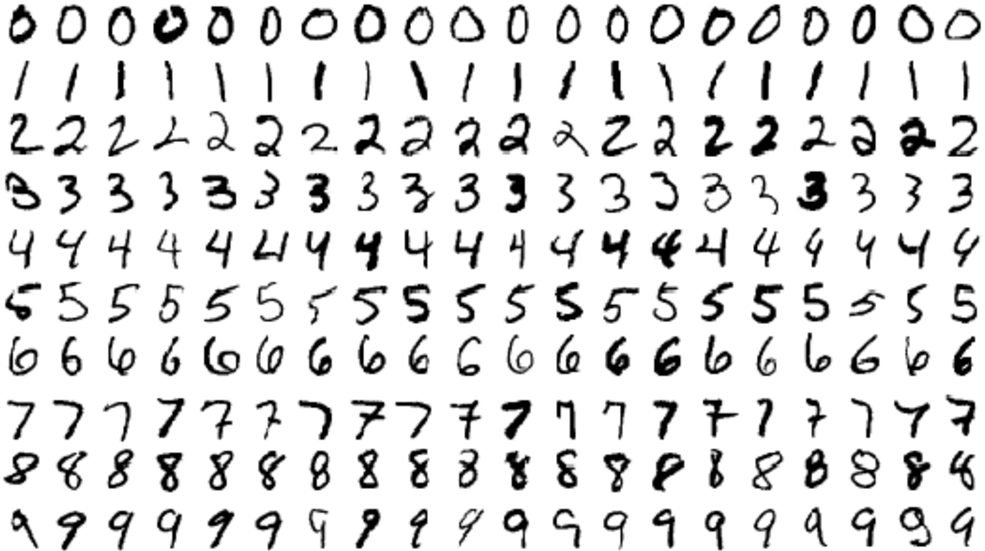
\includegraphics[keepaspectratio, width=0.45\textwidth]{mnist.png}
  \caption{Sample images from MNIST}
\end{figure}

\begin{figure}[t!]
  \centering
  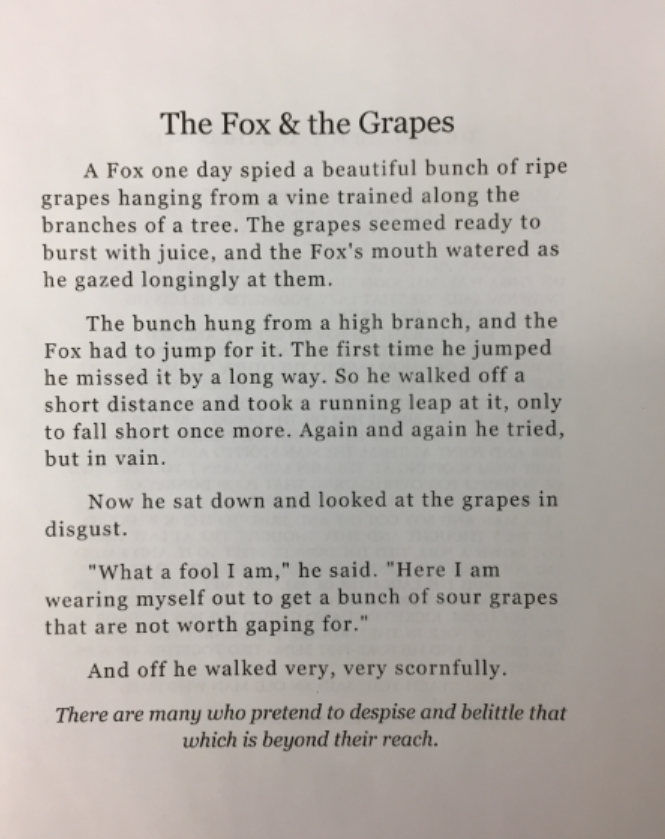
\includegraphics[keepaspectratio, width=0.5\textwidth]{fox.png}
  \caption{Sample typed document {\tt aesop\textunderscore fox.png}}
\end{figure}

\begin{figure}[t!]
  \centering
  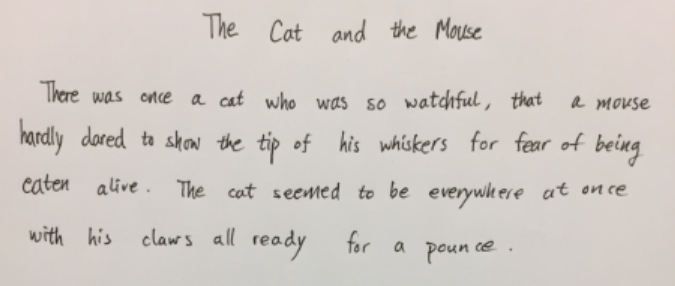
\includegraphics[keepaspectratio, width=0.5\textwidth]{cat.png}
  \caption{Reasonably handwritten doc {\tt hand\textunderscore cat.png}}
\end{figure}

\begin{figure}[t!]
  \centering
  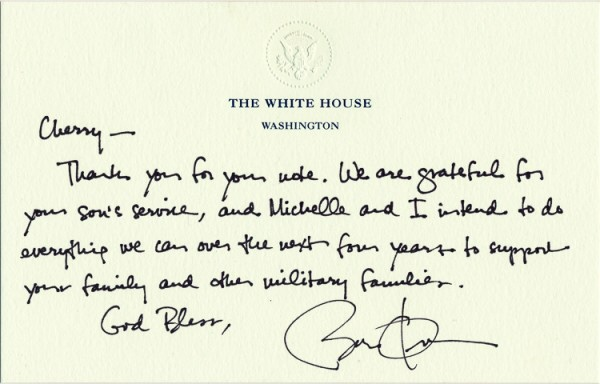
\includegraphics[keepaspectratio, width=0.5\textwidth]{obama4.png}
  \caption{Less neatly handwritten doc {\tt obama1.png}}
\end{figure}

\subsection{Text Translation}

We made use of Google Cloud's Translation API in order to translate the OCR processed document into several different languages based on user command line input. We referred to external code \footnote{http://github.com/mouuff/mtranslate} to make API calls and modified the details to fit our purpose. Moreover, we needed to carefully deal with the translated output in utf-8 when writing them to text files since they were not always simple ASCII.

\subsection{Template Matching}

Aside from OCR, which was the main focus of this project, we also experimented with template matching in images. We tested with various targets. First, we targeted to identify signatures of U.S. Presidents Barack Obama, George W. Bush, and Bill Clinton in documents. Our dataset consisted of handwritten letters written by the presidents as input images and their respective signature images as templates.

Next, we experimented with the JHU logo to determine whether an input document was an official JHU document. We simply assumed that official JHU documents contained a JHU logo for experimental purposes. We used {\tt cv2.matchTemplate} with our input documents as the source image, multiple JHU logo images (each with different sizes since {\tt cv2.matchTemplate} is scale sensitive) as templates, and matching method {\tt cv2.TM\textunderscore CCOEFF\textunderscore NORMED}. If the normazlied {\tt TM\textunderscore CCOEFF} value came out to be greater than 0.51 for any of the input JHU logo templates, we determined that the input document contained a JHU logo in it. The matching method and determinant value of 0.51 were chosen empirically.

\section{Results}

We qualitatively discuss OCR and template matching results on typed and handwritten documents.

\subsection{OCR on Typed Documents}

We ran our code on seven document images with different font types and font sizes. The images were {\tt cv\textunderscore proj\textunderscore description.png}, {\tt cv\textunderscore jchoi\textunderscore proposal.png}, {\tt aesop\textunderscore fox.png}, {\tt lav\textunderscore notes1.png}, {\tt aesop\textunderscore miller.png}, {\tt aesop\textunderscore goose.png}, and {\tt aesop\textunderscore cat.png}. With the exception of {\tt aesop\textunderscore goose.png}, performance on all documents were nearly perfect. Potential reasons of failure with this particular image are discussed in the next section.

\subsection{OCR on Handwritten Documents}

We applied our code on photos of handwritten documents. Performance on very neatly written documents ({\tt hand\textunderscore fox.png} and {\tt hand\textunderscore goose.png}) was nowhere close to what we saw for the printed dataset. Moreover, any reasonably neatly handwritten documents ({\tt hand\textunderscore miller.png} and {\tt hand\textunderscore cat.png}) showed even poorer performance.  Furthermore, our code was not able to detect a single word from document images with much less neat handwriting. Such images were {\tt obama1.png}, {\tt obama2.png}, {\tt obama3.png}, {\tt bush1.png}, {\tt bush2.png}, {\tt clinton1.png}, and {\tt clinton2.png}.

\subsection{Template Matching}

The results for the U.S. presidents' signatures was poor. We then used the JHU logo to determine whether the input document was an official JHU document or not. This experiment showed more promising results. We discuss potential reasons in the next section.

\section{Discussion}

\subsection{Image Processing}

In running our experiments, we tested out with various configurations for denoising and smoothening. Certain parameter configurations worked almost perfectly for some images while they produced disappointing outcome for others. We chose parameter values that performed acceptably well on all images in our dataset. The motivation behind denoising in our work was that document scans usually have many random specs throughout. Such noise can greatly reduce OCR accuracy because an OCR algorithm may confuse a random spec with punctuation marks or associate a spec with an actual character near by. (e.g. confuse an $l$ and ` with an $i$)

\subsection{OCR}

The reason that {\tt aesop\textunderscore goose.png} did not produce satisfactory results was that the font in the document was relatively thick and bold. Therefore, after the preprocessing stage, the alphabet characters in the thresholded document were hollow with just the edges remaining. Therefore, the OCR algorithm could not recognize any of the characters in this text.

The two images {\tt cv\textunderscore jchoi\textunderscore proposal.png} and {\tt lav\textunderscore notes1.png} were taken under sub-optimal conditions: irregular lighting, partial skew, and/or glossy surfaces. We ran our code on these two document images. Moreover, these documents had mixed font types and sizes, and the structure of the document was more complicated than the previous inputs. Despite the less optimal settings, we correctly denoised and thresholded the images and obtained similar results as before.

\subsection{Template Matching}

Performance for this experiment was poor, and we decided to experiment with an easier, rigid template. Performance on the JHU logo template experiments was better compared to that of the U.S. president signature experiments. The reason that the task is harder for the earlier experiment is that the JHU logo is fixed in terms of how it is comprised (lines, curves, color density, etc.) where as signatures vary each time it is signed (penstroke width, curvature, ratio of one part of the signature to another, etc.). Therefore, we think that the ``signature matching task'' bears more resemblance to an object recognition task than an OCR task.

Moreover, we conjecture that the reason that the U.S. president experiment did not work well is that the input documents were handwritten. Therefore, the template matching algorithm could have had more variability to deal with since the entire document contained possible matching candidates. This was apparent when we saw the algorithm output locations of random words within the letters as matches to the signature templates.

\section{Conclusion}

We explored optical character recognition on photographed documents in various settings and formats. We tested with optimal and suboptimal photography settings, experimented with documents with various fonts, and compared performance on typed and handwritten documents. For typed documents, we saw accurate results under both optimal and suboptimal settings even if they contained various font sizes and font types. However, we were not able to achieve accurate results with handwritten document photos, disregarding the neatness of the handwriting. For sufficiently small portions of handwritten documents (e.g. a single word or a short sentence), the OCR algorithm was able to produce correct output occasionally. However, even this was not often enough to be considered reliable. 

Nonetheless, on typed documents, we were able to effectively preprocess the document image and perform OCR on the cleaned data. Moreover, we leveraged the Google Cloud Translation API to translate documents into several different languages. Our final experiments on template matching also deserves future development into a project of its own.

\section*{How to Run the Code}

Please refer to our GitHub repository \footnote{https://github.com/jchoi100/computer\textunderscore vision\textunderscore project}. Assuming that the user has installed all required packages and dependencies, run the following command.\\

\textbf{Command:} \textit{ \$python driver.py \{path-to-image-file\} \{list of target languages separated by space\}}\\

\textbf{Sample usage:} \textit{python driver.py doc7.png es fr ko}\\

The sample command above performs OCR on {\tt doc7.png}, outputs the thresholded image, the text in the original input language, and the text translated in Spanish, French, and Korean.

\section*{Saved Output from Experiments}

Please refer to our GitHub repository.

\section*{Acknowledgments}

We thank the {\tt OpenCV} and {\tt tesseract}, the code we referred to for constructing CNNs using {\tt Keras},  MNIST for the handwritten digit dataset, and Google for the translation API.

We also thank Ji Won Shin (\textit{JHU Class of 2019}) for generously providing the author with a Macbook that could run {\tt tesseract}.

And thanks to Professor Reiter and the TAs for a great semester! Have a great winter break.

\end{document}
